\section{Istniejące rozwiązania}

W ramach pracy przeprowadzono analizę rynkową pod kątem istniejących, ciekawych rozwiązań. Poniżej zaprezentowano trzy najbardziej charakterystyczne z nich.

\begin{itemize}
\item Spark Nano 5.0 GPS Tracker

To przenośne urządzenie do śledzenia pozycji geograficznej przy pomocy systemu GPS posiada zasilane bateryjnie. Zapewnia zdalne powiadamianie użytkownika o lokalizacji urządzenia poprzez sieć CDMA, z dokładnością do 2m. Wymiary urządzenia: 64,5 x 40 x 20,5 mm. Urządzenie pozwala na działanie przez ok. 2 tygodnie, przy założeniu pracy przez 1 godzinę dziennie. Producent udostępnia platformę online oraz aplikacje na smartphony z systemem Android oraz IOS, do przedstawiania danych użytkownikowi.   Urządzenie domyślnie raportuje położenie co minutę, lecz producent umożliwia zdalne zwiększenie częstotliwości w razie chęci użytkownika. Cena urządzenia: 129,99\$. Wizualizację urządzenia przedstawiono na rysunku \ref{fig:image_spark_nano_tracker}.
\begin{figure}[h]
	\centering
	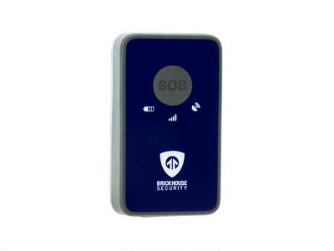
\includegraphics[width=7cm]{img/introduction/spark_nano.jpg}
	\caption{Spark Nano 5.0 GPS Tracker}
	\label{fig:image_spark_nano_tracker}
\end{figure}

\item MyCarTracks - aplikacja mobilna

Jest to aplikacja na smartphona, która dodaje do niego funkcjonalność trackera GPS. Stanowi rozwiązanie typowo programowe, które wykorzystuje zasoby zawarte w telefonie – moduł GPS, GSM oraz internet. Jest ono proste i tanie, lecz nie pozbawione wad. Ponieważ to aplikacja na telefon, a nie osobne urządzenie, konieczne jest umieszczenie smartphone’a w pojeździe na stałe jeśli użytkownik chciałby użytkować ją jako zabezpieczenie antykradzieżowe. Ponadto, telefony pobierają stosunkowo dużo energii co wymusza częste ich ładowanie. W rezultacie efektywne ukrycie urządzenia jest utrudnione. 
Do kosztów rozwiązania należy wliczyć cenę telefonu (używane urządzenie kosztuje ok. 200-300zł) oraz 7\$ za każdy pojazd miesięcznie. Aplikację przedstawiono na rysunku \ref{fig:image_my_car_tracks}.
\begin{figure}[h]
	\centering
	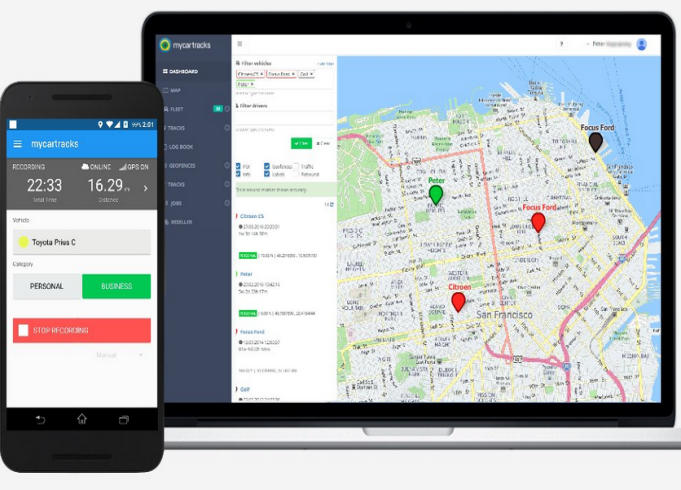
\includegraphics[width=7cm]{img/introduction/mycartracks.jpg}
	\caption{Aplikacja MyCarTracks}
	\label{fig:image_my_car_tracks}
\end{figure}

\item STI GL300

Jest to kolejne niewielkie, przenośne urządzenie wykorzystujące moduł GPS do lokalizacji. Przekazuje ono informacje o położeniu w czasie rzeczywistym (co 60, 10 lub 5 sekund w zależności od wykupionej taryfy). Producent nie przedstawił informacji o sposobie komunikacji z serwerem, lecz najprawdopodobniej również wykorzystuje sieć GSM. Urządzenie to posiada baterię pozwalającą na ciągłą pracę do 2 tygodni. Urządzenie to nie ogranicza się do lokalizacji pojazdów dzięki niewielkim wymiarom. Producent wprowadza ciekawe funkcjonalności: powiadamianie poprzez wiadomość sms o osiągnięciu przez pojazd danej pozycji geograficznej, wejście w zdefiniowany obszar czy osiągnięcie pewnej prędkości. Aktualne oraz historyczne dane są przedstawiane użytkownikowi poprzez stronę internetową na mapach od firmy Google.  Wymiary urządzenia to zaledwie ok. 5 cm x 2,5 cm x 2 cm.  W opcji dodatkowej można dokupić wodoodporną obudowę, pozwalającą na zamontowanie urządzenia na zewnątrz pojazdu. Cena urządzenia to 70\$ oraz od 25\$ do 40\$ miesięcznej opłaty. Wygląd urządzenia pokazano na rysunku \ref{fig:image_sti_gl300}.
\begin{figure}[h]
	\centering
	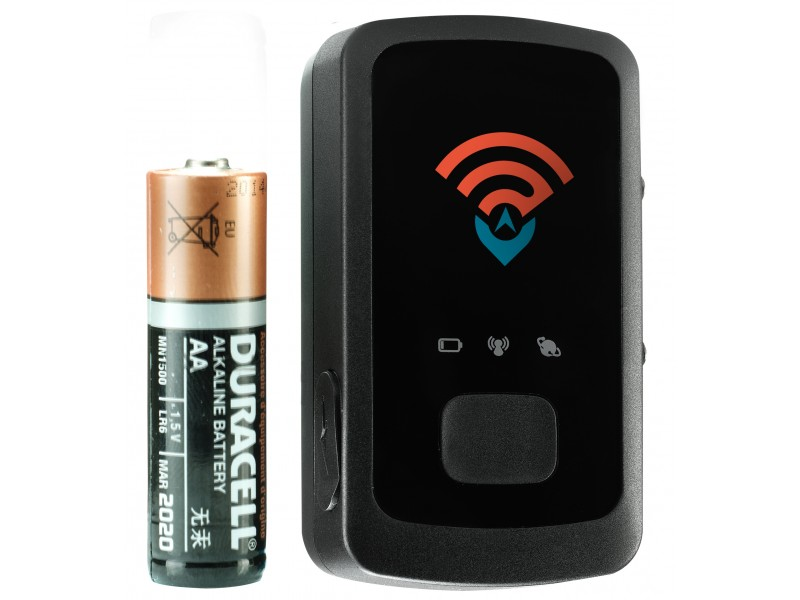
\includegraphics[width=7cm]{img/introduction/sti_gl300.jpg}
	\caption{Urządzenie STI GL300}
	\label{fig:image_sti_gl300}
\end{figure}
\end{itemize}